\section*{問題5}
標本数$n$(コインを投げる回数)を500としたときの$\hat{c}_{\rm min}$の分布のヒストグラムは以下のようになる.
\begin{figure}[H]
    \begin{center}
        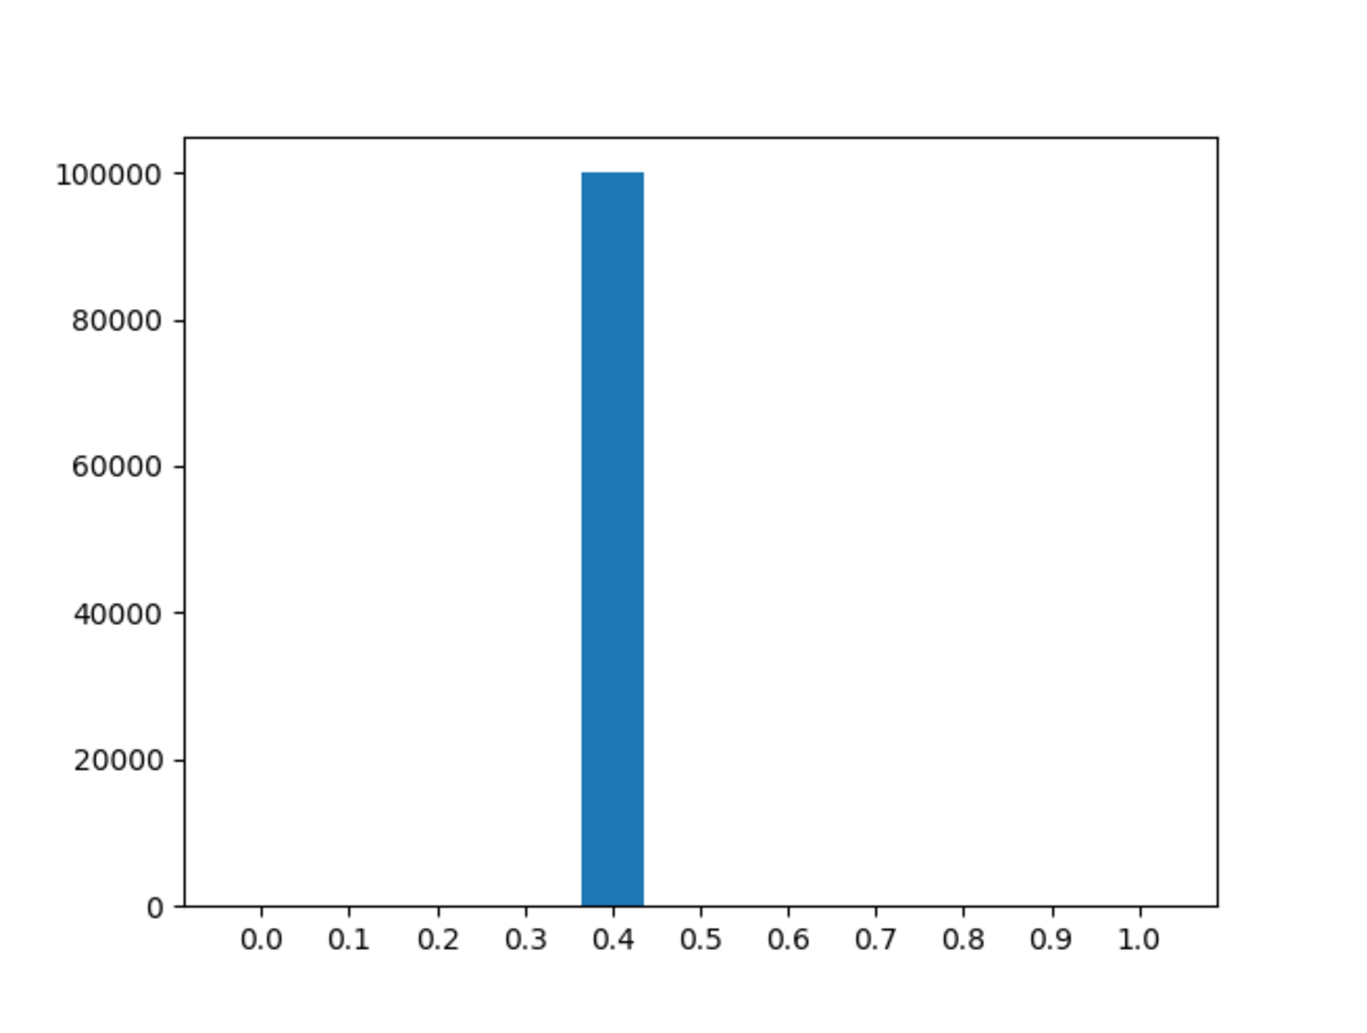
\includegraphics[width=100mm]{./figures/section_5/c_min_500.eps}
        \captionsetup{labelformat=empty,labelsep=none}
        \caption{$\hat{c}_{\rm min}$($n=500$)}
    \end{center}
\end{figure}

標本数が10である問題3の$\hat{c}_{\rm min}$では,分布が$\hat{c}=0.0,\ 0.1$(コインが表である割合)に集まっているのに対して,標本数が500のときは分布が$\hat{c}=0.4$に集まっている.
標本数が10のように少ない場合は,1000枚のコインの中に期待値$\hat{c}=0.5$から大きく外れた$\hat{c}$の非常に小さいコインが紛れている可能性は非常に高い.
しかし,標本数が500のように多い場合は,確率が収束し,$\hat{c}$が最も小さいコインでも期待値から大きく外れず,分布が$\hat{c}=0.4$辺りに集まっていると考えられる.